Após a definição dos parâmetros Cordic é então realizada a implementação da arquitetura do processador em FPGA, através da linguagem VHDL.

Segundo \citeonline{Chih} as operações de multiplicação dos termos SPT, da Equação (\ref{eq:MSR}), podem ser realizadas através de operadores lógicos de deslocamento de \texit(bit), ou  \textit{shifters}. 

 
\vspace{5mm}
\begin{figure}[H]
	\centering
	\captionsetup{width=0.9\textwidth, font=footnotesize, textfont=bf}	
	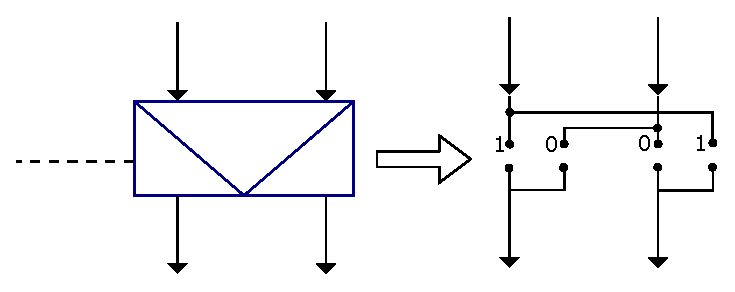
\includegraphics[width=0.3\linewidth]{Images/ImplementandoCordic/Sswitch.eps}
	\caption{Arquitetura Switch 2x2}
	\vspace{-3.5mm}
	\caption*{Fonte: Adaptado \cite{Chih}}
	\label{fig:Sswitch}
\end{figure}    
\vspace{5mm}

\vspace{5mm}
\begin{figure}[H]
	\centering
	\captionsetup{width=0.9\textwidth, font=footnotesize, textfont=bf}	
	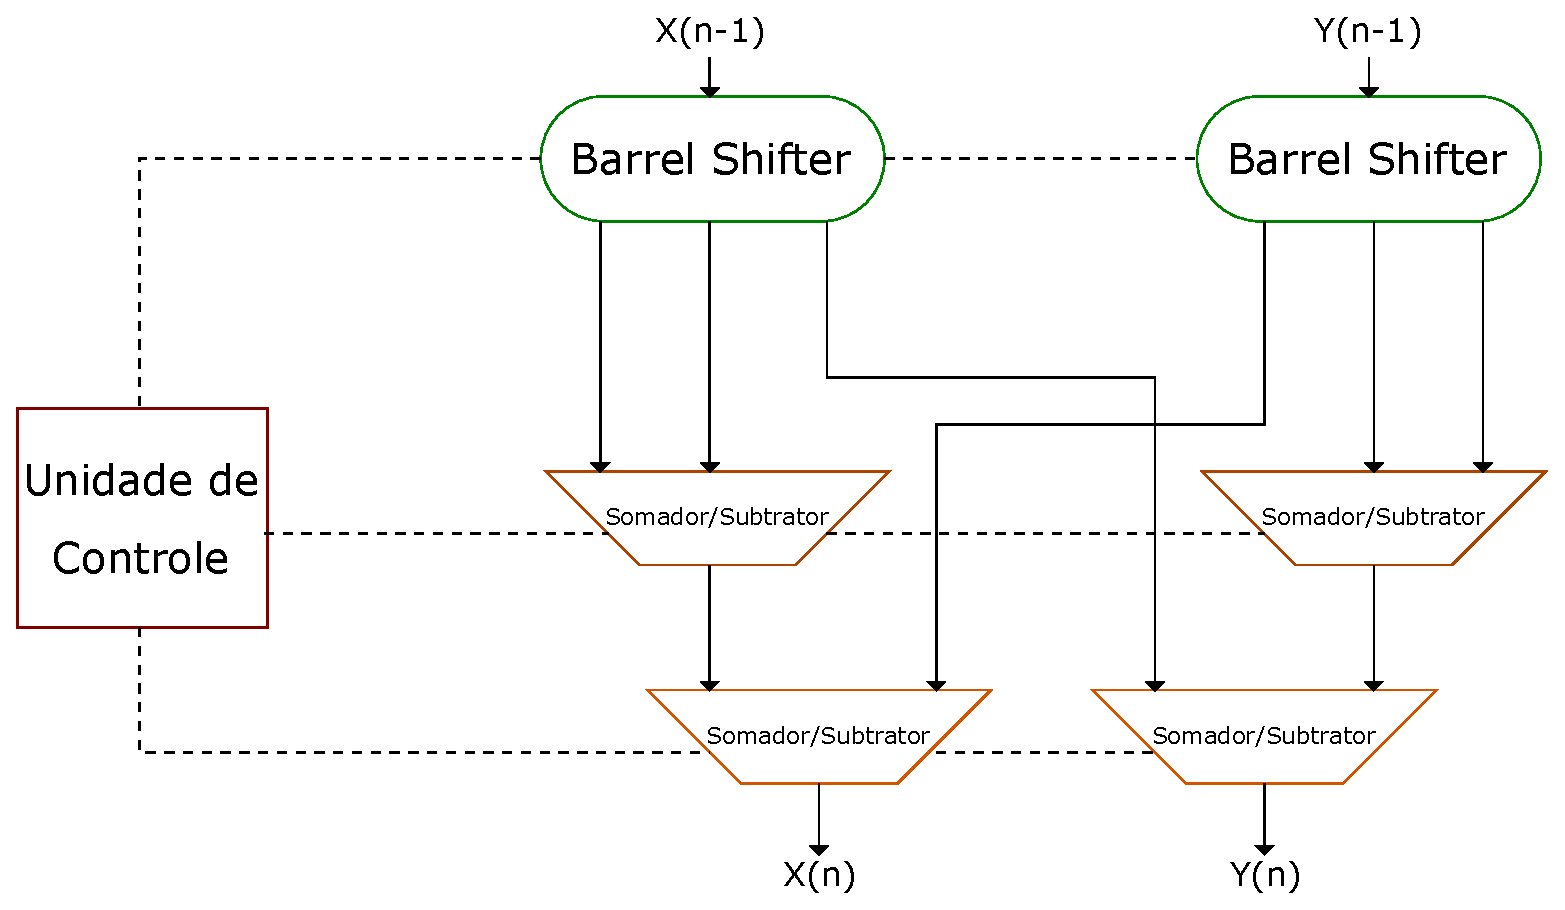
\includegraphics[width=0.9\linewidth]{Images/ImplementandoCordic/ArquiteturaCordicNormal.eps}
	\caption{Arquitetura MSR Cordic Modo Generalizado $N_{spt}=3$}
	\vspace{-3.5mm}
	\caption*{Fonte: Adaptado \cite{Chih}}
	\label{fig:ArquiteturaCordicNormal}
\end{figure}    
\vspace{5mm}

\vspace{5mm}
\begin{figure}[H]
	\centering
	\captionsetup{width=0.9\textwidth, font=footnotesize, textfont=bf}	
	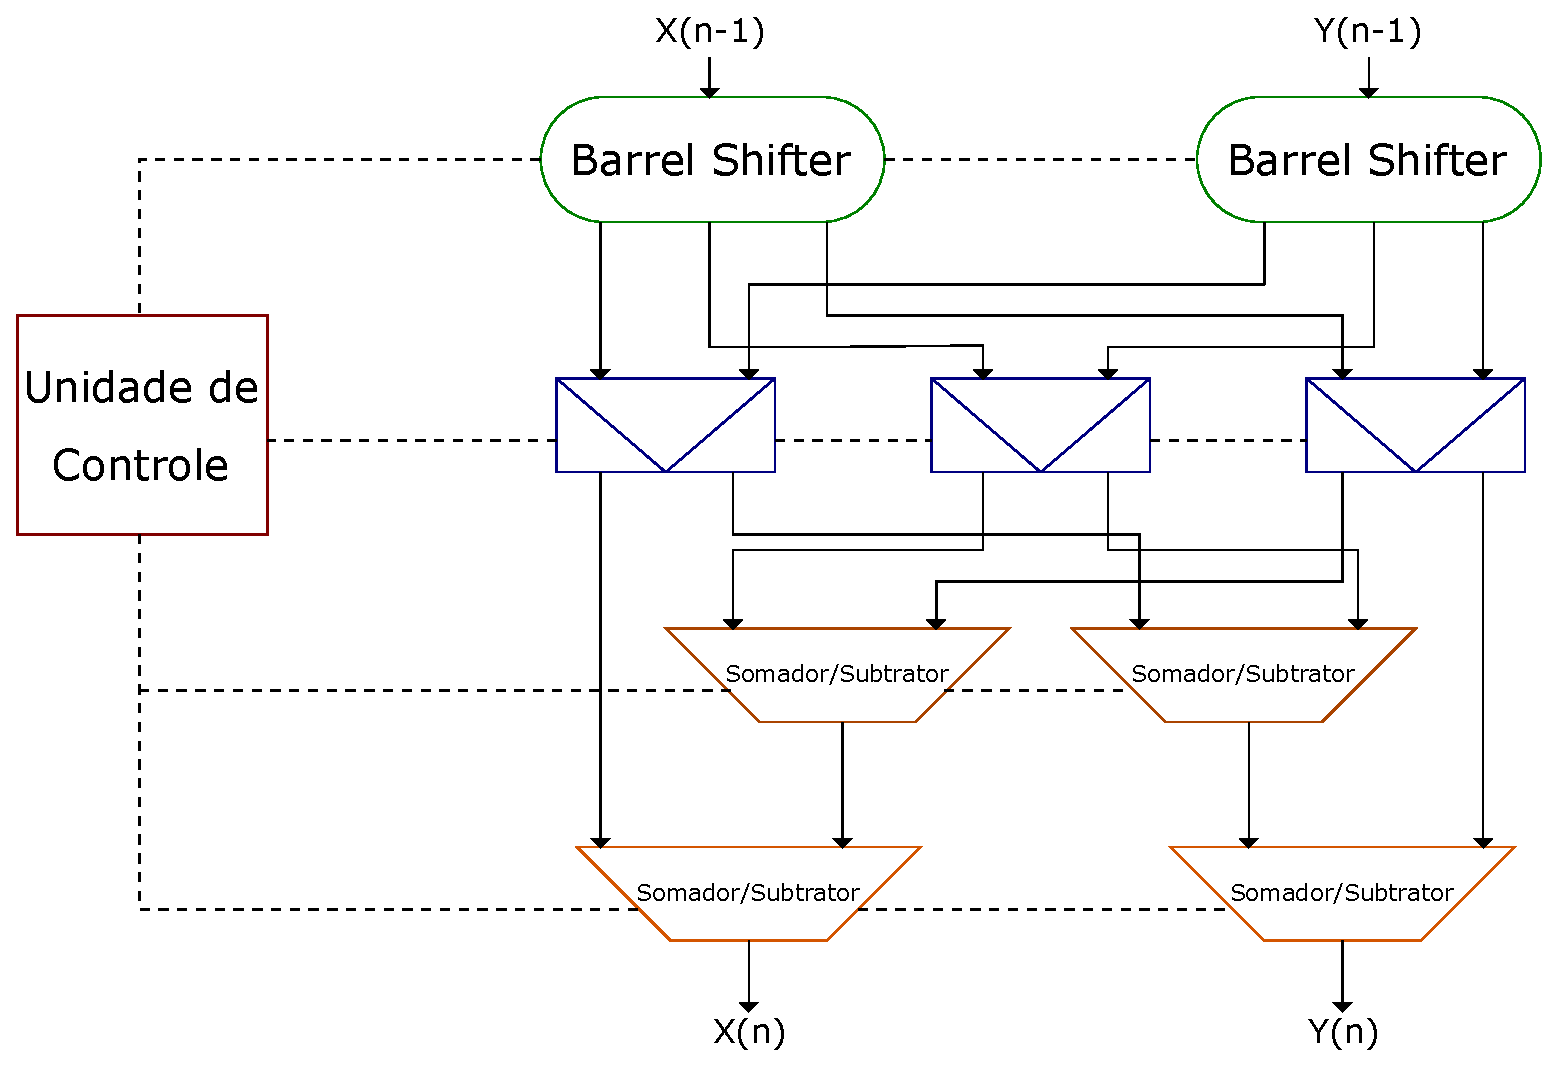
\includegraphics[width=0.9\linewidth]{Images/ImplementandoCordic/ArquiteturaCordicGeneralizado.eps}
	\caption{Arquitetura MSR Cordic Modo Normal $N_{spt}=3$}
	\vspace{-3.5mm}
	\caption*{Fonte: Adaptado \cite{Chih}}
	\label{fig:ArquiteturaCordicGeneralizado}
\end{figure}    
\vspace{5mm}